\documentclass[12pt, titlepage]{article}

\usepackage{fullpage}
\usepackage[round]{natbib}
\usepackage{multirow}
\usepackage{booktabs}
\usepackage{tabularx}
\usepackage{graphicx}
\usepackage{float}
\usepackage{hyperref}
\hypersetup{
    colorlinks,
    citecolor=blue,
    filecolor=black,
    linkcolor=red,
    urlcolor=blue
}

%% Comments

\usepackage{color}

\newif\ifcomments\commentstrue %displays comments
%\newif\ifcomments\commentsfalse %so that comments do not display

\ifcomments
\newcommand{\authornote}[3]{\textcolor{#1}{[#3 ---#2]}}
\newcommand{\todo}[1]{\textcolor{red}{[TODO: #1]}}
\else
\newcommand{\authornote}[3]{}
\newcommand{\todo}[1]{}
\fi

\newcommand{\wss}[1]{\authornote{blue}{SS}{#1}} 
\newcommand{\plt}[1]{\authornote{magenta}{TPLT}{#1}} %For explanation of the template
\newcommand{\an}[1]{\authornote{cyan}{Author}{#1}}

%% Common Parts

\newcommand{\progname}{Software Engineering}
\newcommand{\authname}{Team 1, BANDwidth
\\ Declan Young
\\ Ben Dubois
\\ Nathan Uy
\\ Aidan Mariglia}                

\usepackage{hyperref}
    \hypersetup{colorlinks=true, linkcolor=blue, citecolor=blue, filecolor=blue,
                urlcolor=blue, unicode=false}
    \urlstyle{same}


\newcounter{acnum}
\newcommand{\actheacnum}{AC\theacnum}
\newcommand{\acref}[1]{AC\ref{#1}}

\newcounter{ucnum}
\newcommand{\uctheucnum}{UC\theucnum}
\newcommand{\uref}[1]{UC\ref{#1}}

\newcounter{mnum}
\newcommand{\mthemnum}{M\themnum}
\newcommand{\mref}[1]{M\ref{#1}}

\begin{document}

\title{Module Guide for \progname{}} 
\author{\authname}
\date{\today}

\maketitle

\pagenumbering{roman}

\section{Revision History}

\begin{tabularx}{\textwidth}{p{3cm}p{2cm}X}
\toprule {\bf Date} & {\bf Version} & {\bf Notes}\\
\midrule
01/07/2025 & 0.1 & revision 0 design\\
\bottomrule
\end{tabularx}

\newpage

\section{Reference Material}

This section records information for easy reference.

\subsection{Abbreviations and Acronyms}

\renewcommand{\arraystretch}{1.2}
\begin{tabular}{l l} 
  \toprule		
  \textbf{symbol} & \textbf{description}\\
  \midrule 
  AC & Anticipated Change\\
  DAG & Directed Acyclic Graph \\
  M & Module \\
  MG & Module Guide \\
  OS & Operating System \\
  R & Requirement\\
  SC & Scientific Computing \\
  SRS & Software Requirements Specification\\
  \progname & Explanation of program name\\
  UC & Unlikely Change \\
  \bottomrule
\end{tabular}\\

\newpage

\tableofcontents

\listoftables

\listoffigures

\newpage

\pagenumbering{arabic}

\section{Introduction}

Decomposing a system into modules is a commonly accepted approach to developing
software.  A module is a work assignment for a programmer or programming
team~\citep{ParnasEtAl1984}.  We advocate a decomposition
based on the principle of information hiding~\citep{Parnas1972a}.  This
principle supports design for change, because the ``secrets'' that each module
hides represent likely future changes.  Design for change is valuable in SC,
where modifications are frequent, especially during initial development as the
solution space is explored.  

Our design follows the rules layed out by \citet{ParnasEtAl1984}, as follows:
\begin{itemize}
\item System details that are likely to change independently should be the
  secrets of separate modules.
\item Each data structure is implemented in only one module.
\item Any other program that requires information stored in a module's data
  structures must obtain it by calling access programs belonging to that module.
\end{itemize}

After completing the first stage of the design, the Software Requirements
Specification (SRS), the Module Guide (MG) is developed~\citep{ParnasEtAl1984}. The MG
specifies the modular structure of the system and is intended to allow both
designers and maintainers to easily identify the parts of the software.  The
potential readers of this document are as follows:

\begin{itemize}
\item New project members: This document can be a guide for a new project member
  to easily understand the overall structure and quickly find the
  relevant modules they are searching for.
\item Maintainers: The hierarchical structure of the module guide improves the
  maintainers' understanding when they need to make changes to the system. It is
  important for a maintainer to update the relevant sections of the document
  after changes have been made.
\item Designers: Once the module guide has been written, it can be used to
  check for consistency, feasibility, and flexibility. Designers can verify the
  system in various ways, such as consistency among modules, feasibility of the
  decomposition, and flexibility of the design.
\end{itemize}

The rest of the document is organized as follows. Section
\ref{SecChange} lists the anticipated and unlikely changes of the software
requirements. Section \ref{SecMH} summarizes the module decomposition that
was constructed according to the likely changes. Section \ref{SecConnection}
specifies the connections between the software requirements and the
modules. Section \ref{SecMD} gives a detailed description of the
modules. Section \ref{SecTM} includes two traceability matrices. One checks
the completeness of the design against the requirements provided in the SRS. The
other shows the relation between anticipated changes and the modules. Section
\ref{SecUse} describes the use relation between modules. Section
\ref{UI} includes the screenshots of the User Interface. Section \ref{Timeline} includes a link to the tasks related to the design, who it is assigned to and the expected completion time.

\section{Anticipated and Unlikely Changes} \label{SecChange}

This section lists possible changes to the system. According to the likeliness
of the change, the possible changes are classified into two
categories. Anticipated changes are listed in Section \ref{SecAchange}, and
unlikely changes are listed in Section \ref{SecUchange}.

\subsection{Anticipated Changes} \label{SecAchange}

Anticipated changes are the source of the information that is to be hidden
inside the modules. Ideally, changing one of the anticipated changes will only
require changing the one module that hides the associated decision. The approach
adapted here is called design for
change.

\begin{description}
\item[\refstepcounter{acnum} \actheacnum \label{acTest}:] The tests and test data that the Matlab models are being tested against
\item[\refstepcounter{acnum} \actheacnum \label{acLeaderboard}:] The categories in the leaderboard
\item[\refstepcounter{acnum} \actheacnum \label{acDisplay}:] How the models' performance is displayed to the user
\item[\refstepcounter{acnum} \actheacnum \label{acExecute}:] How the model is executed e.g. execution progress reports, error handling, etc. 
\item[\refstepcounter{acnum} \actheacnum \label{acLanguage}:] The programming language of the models submitted by the user
\end{description}

\subsection{Unlikely Changes} \label{SecUchange}

The module design should be as general as possible. However, a general system is
more complex. Sometimes this complexity is not necessary. Fixing some design
decisions at the system architecture stage can simplify the software design. If
these decision should later need to be changed, then many parts of the design
will potentially need to be modified. Hence, it is not intended that these
decisions will be changed.

\begin{description}
\item[\refstepcounter{ucnum} \uctheucnum \label{ucIO}:] Input/Output devices
  (Input: file, mouse, keyboard, Output: monitor screen).
\item[\refstepcounter{ucnum} \uctheucnum \label{ucIO}:] User log-in
\item[\refstepcounter{ucnum} \uctheucnum
\label{ucIO}:] Database Management System
\item[\refstepcounter{ucnum} \uctheucnum
\label{ucIO}:] API Communication
\end{description}

\section{Module Hierarchy} \label{SecMH}

This section provides an overview of the module design. Modules are summarized
in a hierarchy decomposed by secrets in Table \ref{TblMH}. The modules listed
below, which are leaves in the hierarchy tree, are the modules that will
actually be implemented.

\begin{description}
\item [\refstepcounter{mnum} \mthemnum \label{mHH}:] Hardware Hiding Module
\item [\refstepcounter{mnum} \mthemnum \label{mA}:] App Module
\item [\refstepcounter{mnum} \mthemnum \label{mUA}:] User Authentication Module
\item [\refstepcounter{mnum} \mthemnum \label{mLI}:] Login Module
\item [\refstepcounter{mnum} \mthemnum \label{mRG}:] Registration Module
\item [\refstepcounter{mnum} \mthemnum \label{mDM}:] Database Management Module
\item [\refstepcounter{mnum} \mthemnum \label{mWS}:] Web Server Module
\item [\refstepcounter{mnum} \mthemnum \label{mI}:] Intro Module
\item [\refstepcounter{mnum} \mthemnum \label{mH}:] Home Module
\item [\refstepcounter{mnum} \mthemnum \label{mME}:] Model Execution Module
\item [\refstepcounter{mnum} \mthemnum \label{mTD}:] Test Data Module
\item [\refstepcounter{mnum} \mthemnum \label{mTA}:] Test Algorithm Module
\item [\refstepcounter{mnum} \mthemnum \label{mS}:] Submit Module
\item [\refstepcounter{mnum} \mthemnum \label{mSN}:] Submission Module
\item [\refstepcounter{mnum} \mthemnum \label{mL}:] Leaderboard Module
\item [\refstepcounter{mnum} \mthemnum \label{mR}:] Results Module
\item [\refstepcounter{mnum} \mthemnum \label{mACP}:] Admin Control Panel Module



\end{description}


\begin{table}[H]
\centering
\begin{tabular}{p{0.3\textwidth} p{0.6\textwidth}}
\toprule
\textbf{Level 1} & \textbf{Level 2}\\
\midrule

{Hardware-Hiding Module}
& \mref{mHH}\\
\midrule

\multirow{10}{0.3\textwidth}{Behaviour-Hiding Module} 
& \mref{mLI}\\
& \mref{mRG}\\
& \mref{mI}\\
& \mref{mH}\\
& \mref{mTA}\\
& \mref{mS}\\
& \mref{mSN}\\
& \mref{mL}\\
& \mref{mR}\\
& \mref{mACP}\\
\midrule

\multirow{6}{0.3\textwidth}{Software Decision Module} 
& \mref{mA}\\
& \mref{mUA}\\
& \mref{mDM}\\
& \mref{mWS}\\
& \mref{mME}\\
& \mref{mTD}\\
\bottomrule

\end{tabular}
\caption{Module Hierarchy}
\label{TblMH}
\end{table}

\section{Connection Between Requirements and Design} \label{SecConnection}

The design of the system is intended to satisfy the requirements developed in
the SRS. In this stage, the system is decomposed into modules. The connection
between requirements and modules is listed in Table~\ref{TblRT}.

\section{Module Decomposition} \label{SecMD}

Modules are decomposed according to the principle of ``information hiding''
proposed by \citet{ParnasEtAl1984}. The \emph{Secrets} field in a module
decomposition is a brief statement of the design decision hidden by the
module. The \emph{Services} field specifies \emph{what} the module will do
without documenting \emph{how} to do it. For each module, a suggestion for the
implementing software is given under the \emph{Implemented By} title. If the
entry is \emph{OS}, this means that the module is provided by the operating
system or by standard programming language libraries.  \emph{\progname{}} means the
module will be implemented by the \progname{} software.

Only the leaf modules in the hierarchy have to be implemented. If a dash
(\emph{--}) is shown, this means that the module is not a leaf and will not have
to be implemented.

\subsection{Hardware Hiding Modules (\mref{mHH})}

\begin{description}
\item[Secrets:]The data structure and algorithm used to implement the virtual
  hardware.
\item[Services:]Serves as a virtual hardware used by the rest of the
  system. This module provides the interface between the hardware and the
  software. So, the system can use it to display outputs or to accept inputs.
\item[Implemented By:] OS
\end{description}

\subsection{Behaviour-Hiding Module}

\begin{description}
\item[Secrets:]The contents of the required behaviours.
\item[Services:]Includes programs that provide externally visible behaviour of
  the system as specified in the software requirements specification (SRS)
  documents. This module serves as a communication layer between the
  hardware-hiding module and the software decision module. The programs in this
  module will need to change if there are changes in the SRS.
\item[Implemented By:] Software Engineering
\end{description}

\subsubsection{Login Module (\mref{mLI})}

\begin{description}
\item[Secrets:] Display logic.
\item[Services:] Render the login page and authentication messages
\item[Implemented By:] Login
\item[Type of Module:] Abstract Object
\end{description}

\subsubsection{Registration Module (\mref{mRG})}

\begin{description}
\item[Secrets:] Display logic.
\item[Services:] Render registration page and authentication messages
\item[Implemented By:] Registration
\item[Type of Module:] Abstract Object
\end{description}

\subsubsection{Intro Module (\mref{mI})}

\begin{description}
\item[Secrets:] Display logic.
\item[Services:] Render intro page
\item[Implemented By:] Intro
\item[Type of Module:] Abstract Object
\end{description}

\subsubsection{Home Module (\mref{mH})}

\begin{description}
\item[Secrets:] Display logic.
\item[Services:] Render home page
\item[Implemented By:] Home
\item[Type of Module:] Abstract Object
\end{description}

\subsubsection{Test Algorithm Module (\mref{mTA})}

\begin{description}
\item[Secrets:] The test algorithm
\item[Services:] Executes tests on the submitted models and evaluates results
\item[Implemented By:] TestAlgorithm
\item[Type of Module:] Abstract Data Type
\end{description}

\subsubsection{Submit Module (\mref{mS})}

\begin{description}
\item[Secrets:] Display logic and error handling.
\item[Services:] Render the submit model page and accept only Matlab files
\item[Implemented By:] Submit
\item[Type of Module:] Abstract Object
\end{description}

\subsubsection{Submission Module (\mref{mSN})}

\begin{description}
\item[Secrets:] Display logic.
\item[Services:] Render a model's detailed result including graphical representations
\item[Implemented By:] Submission
\item[Type of Module:] Abstract Object
\end{description}

\subsubsection{Leaderboard Module (\mref{mL})}

\begin{description}
\item[Secrets:] Sorting/Filtering Algorithm choice
\item[Services:] Displays results of previous submissions, provides sorting and filtering options
\item[Implemented By:] Leaderboard
\item[Type of Module:] library
\end{description}

\subsubsection{Results Module (\mref{mR})}

\begin{description}
\item[Secrets:] Display logic.
\item[Services:] Render all user's submission results
\item[Implemented By:] Result
\item[Type of Module:] Abstract Object
\end{description}

\subsubsection{Admin Control Panel Module (\mref{mACP})}

\begin{description}
\item[Secrets:] Admin related logic
\item[Services:] Authorization and Execution of admin actions, 
\item[Implemented By:] django.contrib.admin
\item[Type of Module:] Library
\end{description}


\subsection{Software Decision Module}

\begin{description}
\item[Secrets:] The design decision based on mathematical theorems, physical
  facts, or programming considerations. The secrets of this module are
  \emph{not} described in the SRS.
\item[Services:] Includes data structure and algorithms used in the system that
  do not provide direct interaction with the user. 
  % Changes in these modules are more likely to be motivated by a desire to
  % improve performance than by externally imposed changes.
\item[Implemented By:] Software Engineering
\end{description}

\subsubsection{App Module (\mref{mA})}

\begin{description}
\item[Secrets:] All secrets of child modules
\item[Services:] Implement all requirements
\item[Implemented By:] All modules
\item[Type of Module:] Library
\end{description}

\subsubsection{User Authentication Module (\mref{mUA})}

\begin{description}
\item[Secrets:] Logic for authentication mechanism and password management. 
\item[Services:] User login/logout, User registration, password recovery/reset.
\item[Implemented By:] django.contrib.auth
\item[Type of Module:] Library
\end{description}

\subsubsection{Database Management Module (\mref{mDM})}

\begin{description}
\item[Secrets:]The types and structure of retained data. The storage and access methods for retained data
\item[Services:]Stores and retrieves data which needs to be retained long term.
\item[Implemented By:] Postgresql and data library.
\item[Type of Module:] Library
\end{description}

\subsubsection{Web Server Module (\mref{mWS})}

\begin{description}
\item[Secrets:] Routing of modules
\item[Services:] Handle routing of requests
\item[Implemented By:] Web Server
\item[Type of Module:] Abstract Object
\end{description}

\subsubsection{Model Execution Module (\mref{mME})}

\begin{description}
\item[Secrets:] Method of executing model. 
\item[Services:] Executing use submitted models against the test suite.
\item[Implemented By:] Matlab
\item[Type of Module:] Library
\end{description}

\subsubsection{Test Data Module (\mref{mTD})}

\begin{description}
\item[Secrets:] The test data's format.
\item[Services:] Provides the data that the model will be tested against.
\item[Implemented By:] TestData
\item[Type of Module:] Record
\end{description}

\section{Traceability Matrix} \label{SecTM}

This section shows two traceability matrices: between the modules and the
requirements and between the modules and the anticipated changes.

% the table should use mref, the requirements should be named, use something
% like fref
\begin{table}[H]
\centering
\begin{tabular}{p{0.2\textwidth} p{0.6\textwidth}}
\toprule
\textbf{Req.} & \textbf{Modules}\\
\midrule
FR1 & \mref{mWS}, \mref{mS}\\
FR2 & \mref{mWS}, \mref{mTD}, \mref{mTA}, \mref{mSN}\\
FR3 & \mref{mME}\\
FR4 & \mref{mWS}, \mref{mRG}\\
FR5 & \mref{mWS}, \mref{mLI}\\
FR6 & \mref{mUA}, \mref{mDM}\\
FR7 & \mref{mDM}\\
FR8 & \mref{mUA}, \mref{mWS}, \mref{mL}\\
FR9 & \mref{mL}\\
FR10 & \mref{mL}\\
FR11 & \mref{mWS}, \mref{mME}, \mref{mR}\\
FR12 & \mref{mWS}, \mref{mME}, \mref{mR}\\
LR1 & \mref{mI}, \mref{mH} \\
LR2 & \mref{mI}, \mref{mH}\\
UPR4 & \mref{mI}, \mref{mH}\\
SLR1 & \mref{mSN}\\
SLR2 & \mref{mL}\\
SLR3 & \mref{mL}\\
RR1 & \mref{mME}\\
IR1 & \mref{mDM}\\
IMR1 & \mref{mUA}\\
\bottomrule
\end{tabular}
\caption{Trace Between Requirements and Modules}
\label{TblRT}
\end{table}

\begin{table}[H]
\centering
\begin{tabular}{p{0.2\textwidth} p{0.6\textwidth}}
\toprule
\textbf{AC} & \textbf{Modules}\\
\midrule
\acref{acTest} & \mref{mTD}, \mref{mTA}\\
\acref{acLeaderboard} & \mref{mL}\\
\acref{acDisplay} & \mref{mS},\mref{mSN}\\
\acref{acExecute} & \mref{mME}\\
\acref{acLanguage} & \mref{mME}\\
\bottomrule
\end{tabular}
\caption{Trace Between Anticipated Changes and Modules}
\label{TblACT}
\end{table}

\section{Use Hierarchy Between Modules} \label{SecUse}

In this section, the uses hierarchy between modules is
provided. \citet{Parnas1978} said of two programs A and B that A {\em uses} B if
correct execution of B may be necessary for A to complete the task described in
its specification. That is, A {\em uses} B if there exist situations in which
the correct functioning of A depends upon the availability of a correct
implementation of B.  Figure \ref{FigUH} illustrates the use relation between
the modules. It can be seen that the graph is a directed acyclic graph
(DAG). Each level of the hierarchy offers a testable and usable subset of the
system, and modules in the higher level of the hierarchy are essentially simpler
because they use modules from the lower levels.

\begin{figure}[H]
\centering
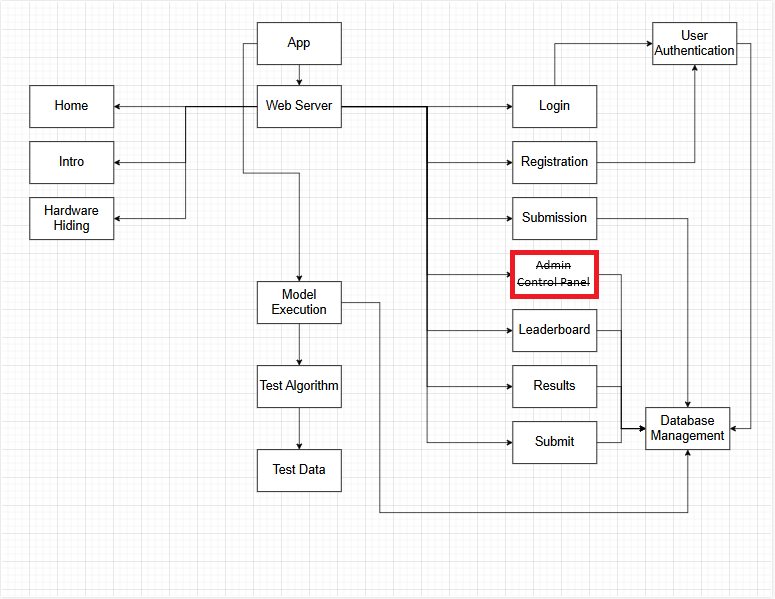
\includegraphics[width=0.7\textwidth]{Use_Hierarchy.png}
\caption{Use hierarchy among modules}
\label{FigUH}
\end{figure}

%\section*{References}

\section{User Interfaces} \label{UI}

Refer to Appendix 1 - 10 (\ref{Appendix}) for screenshots of the various views for the design of the User Interface.

\begin{itemize}
    \item \ref{Appendix 1}: Intro Page
    \item \ref{Appendix 2}: Registration Page
    \item \ref{Appendix 3}: Login Page
    \item \ref{Appendix 4}: Home Page
    \item \ref{Appendix 5}: Submit Page
    \item \ref{Appendix 6}: Results Page
    \item \ref{Appendix 7}: Submission Page
    \item \ref{Appendix 8}: Leaderboard Page
    \item \ref{Appendix 9}: Leaderboard Page (with sorting)
    \item \ref{Appendix 10}: Leaderboard Page (with filtering)
\end{itemize}

\section{Timeline} \label{Timeline}

Refer to the Project Board to view all tasks related to the design described in this document - \url{https://github.com/users/AidanMariglia/projects/1}.\\ \\ All tasks explain the necessary work for completion as well as who is responsible for the task.

\section{Appendix}\label{Appendix}

\subsection{Appendix 1} \label{Appendix 1}
\begin{figure}[H]
    \centering
    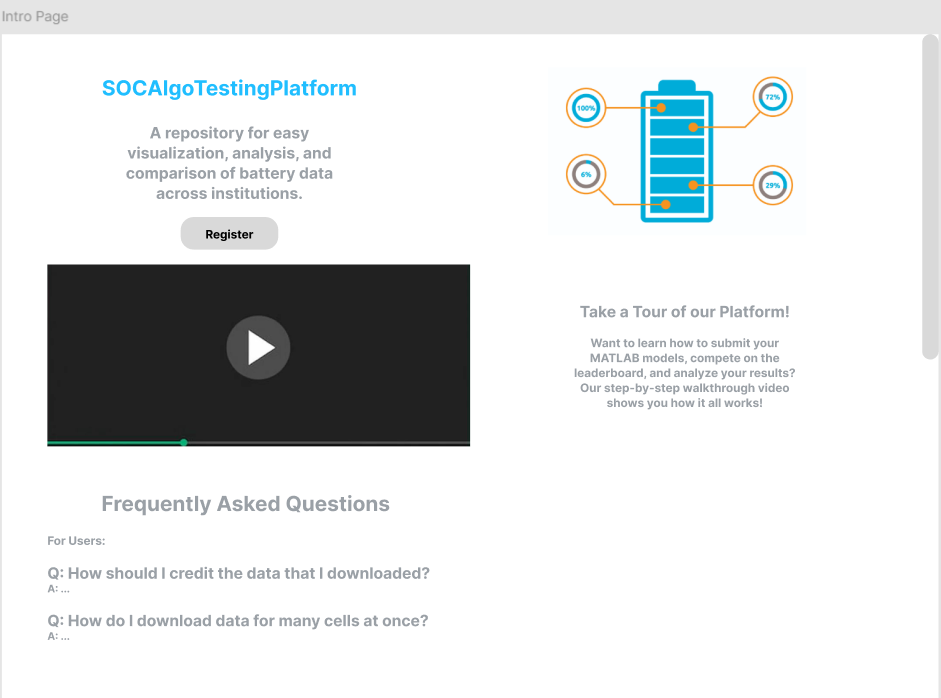
\includegraphics[width=1\linewidth]{.//Interface/Intro.png}
\end{figure}
\subsection{Appendix 2} \label{Appendix 2}
\begin{figure}[H]
    \centering
    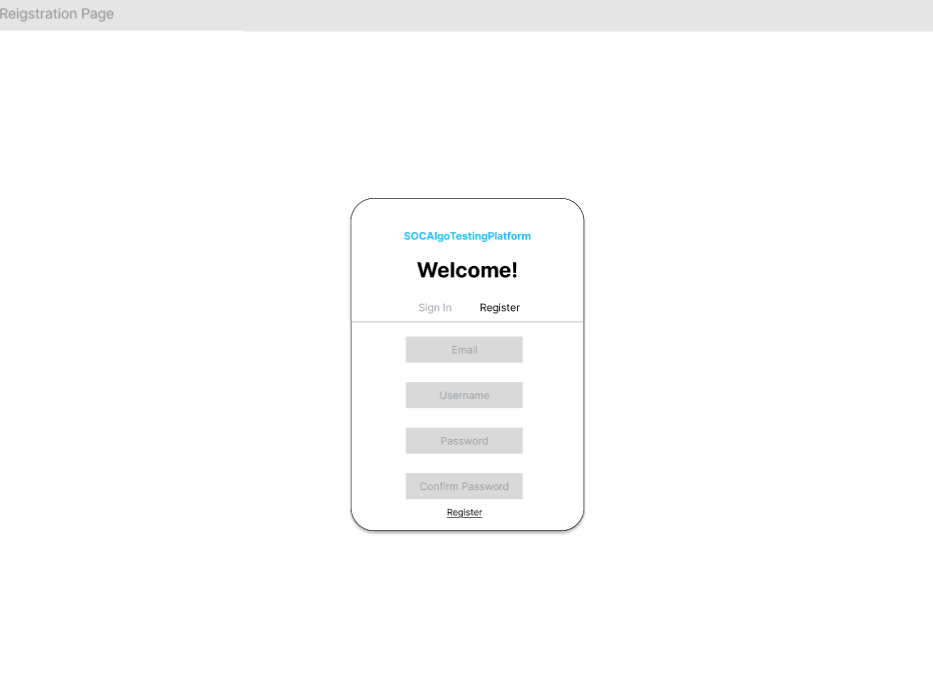
\includegraphics[width=1\linewidth]{.//Interface/Registration.png}
\end{figure}
\subsection{Appendix 3} \label{Appendix 3}
\begin{figure}[H]
    \centering
    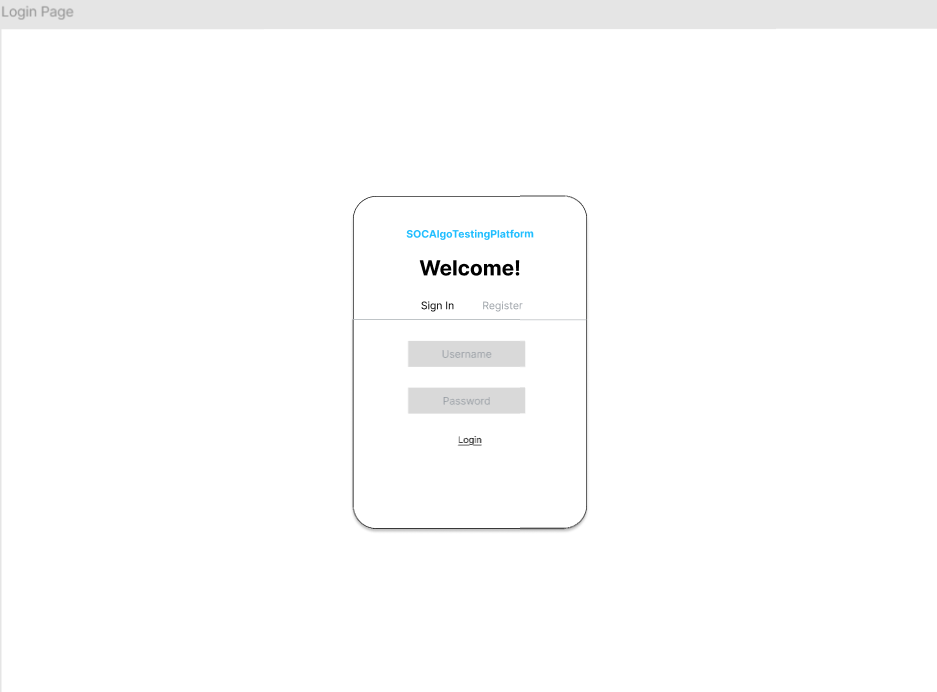
\includegraphics[width=1\linewidth]{.//Interface/Login.png}
\end{figure}
\subsection{Appendix 4} \label{Appendix 4}
\begin{figure}[H]
    \centering
    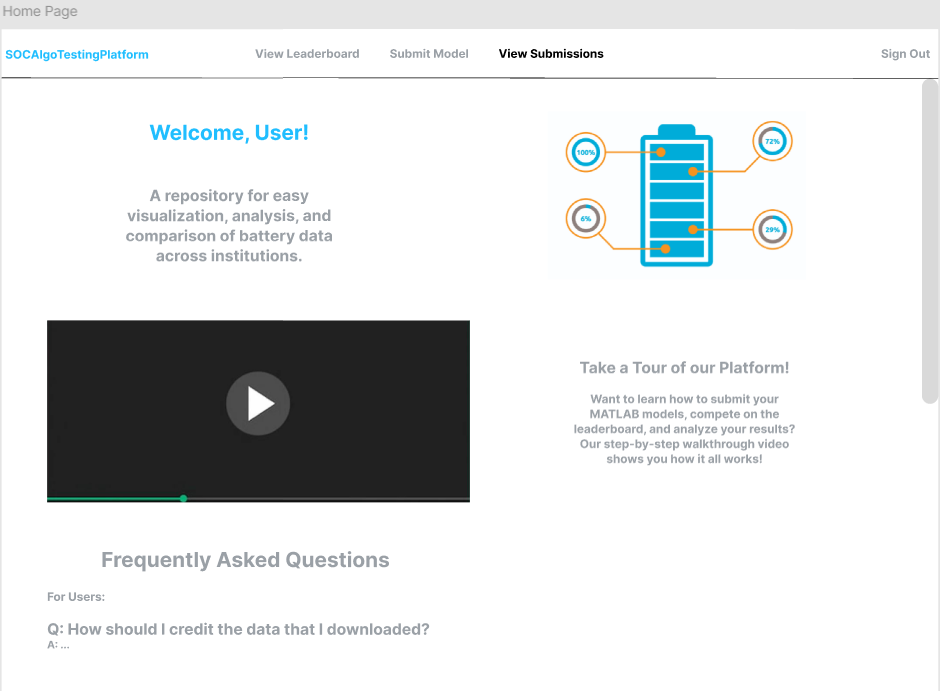
\includegraphics[width=1\linewidth]{Interface/Home.png}
\end{figure}
\subsection{Appendix 5} \label{Appendix 5}
\begin{figure}[H]
    \centering
    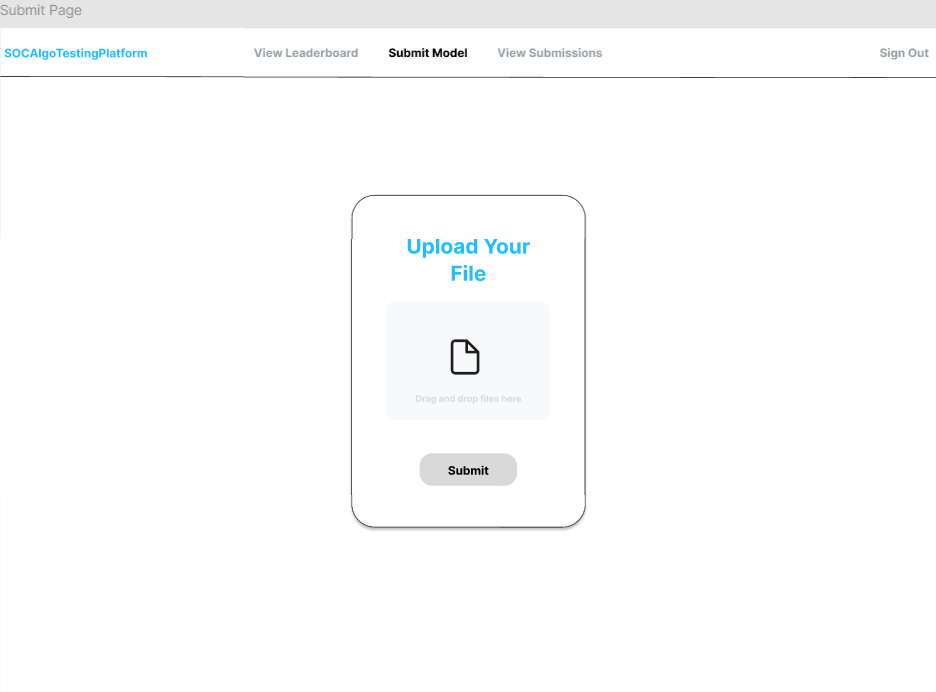
\includegraphics[width=1\linewidth]{.//Interface/Submit.png}
\end{figure}
\subsection{Appendix 6} \label{Appendix 6}
\begin{figure}[H]
    \centering
    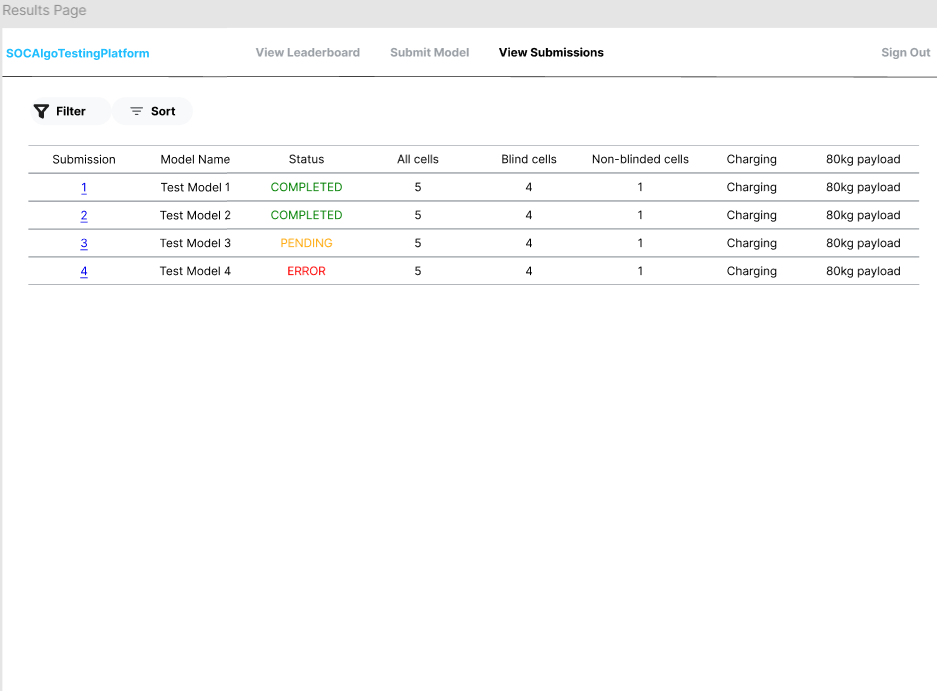
\includegraphics[width=1\linewidth]{.//Interface/Results.png}
\end{figure}
\subsection{Appendix 7} \label{Appendix 7}
\begin{figure}[H]
    \centering
    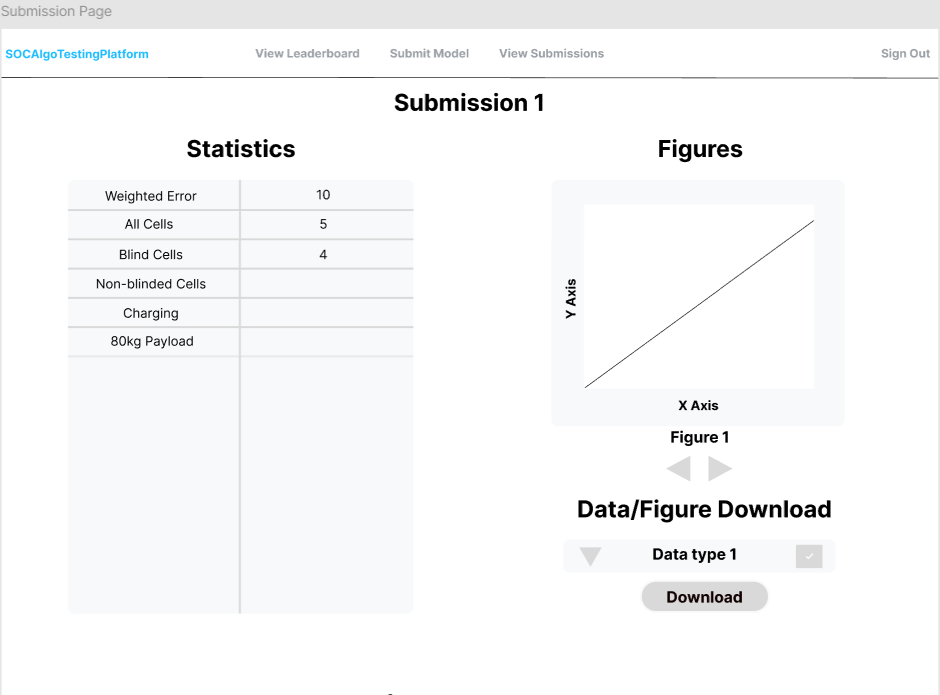
\includegraphics[width=1\linewidth]{.//Interface/Submission.png}
\end{figure}
\subsection{Appendix 8} \label{Appendix 8}
\begin{figure}[H]
    \centering
    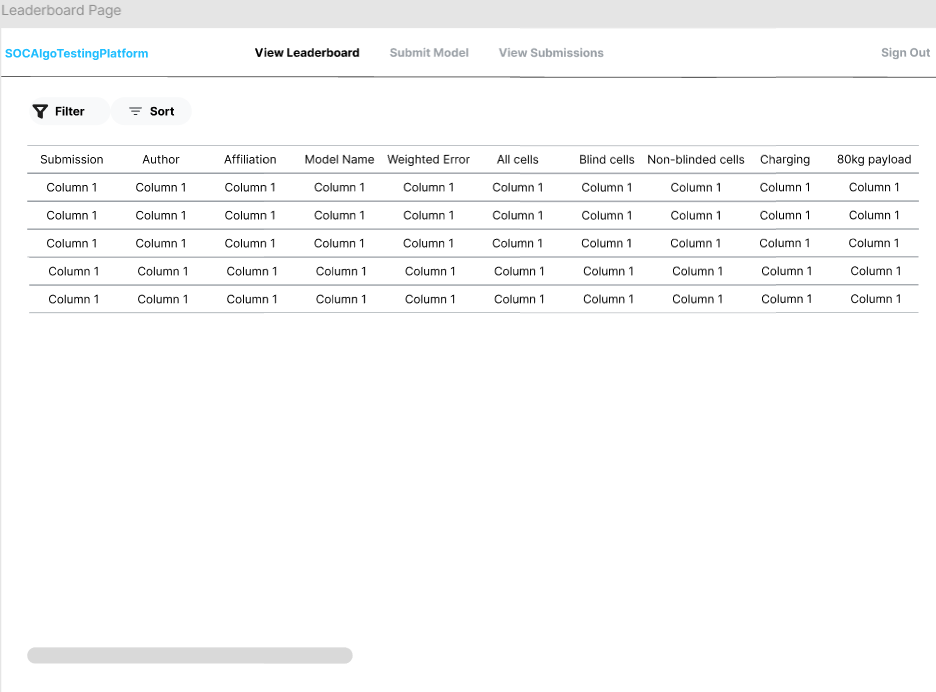
\includegraphics[width=1\linewidth]{.//Interface/Leaderboard.png}
\end{figure}
\subsection{Appendix 9} \label{Appendix 9}
\begin{figure}[H]
    \centering
    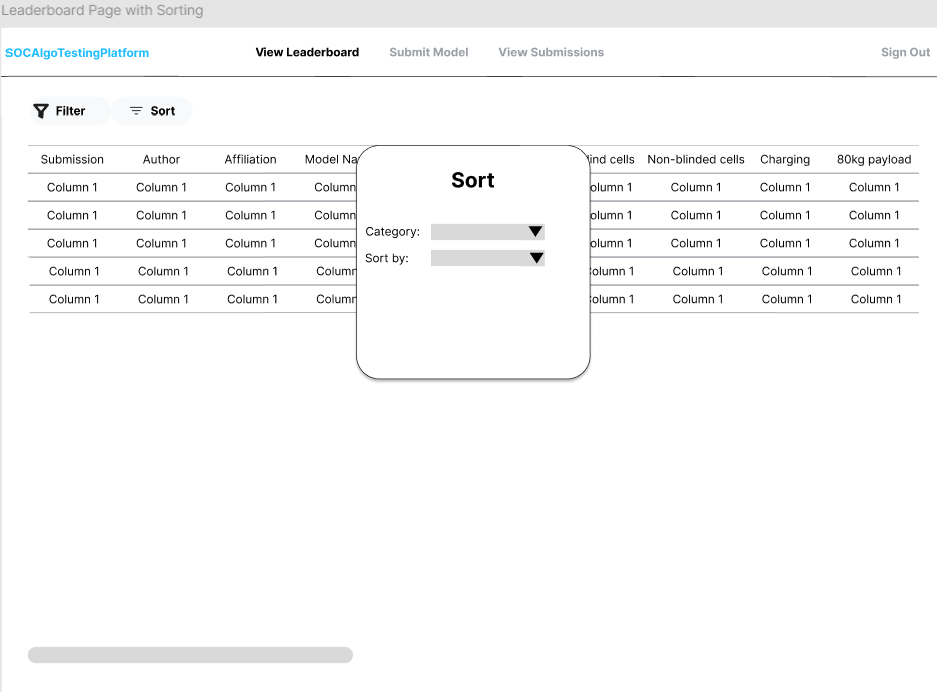
\includegraphics[width=1\linewidth]{.//Interface/Sorting.png}
\end{figure}
\subsection{Appendix 10} \label{Appendix 10}
\begin{figure}[H]
    \centering
    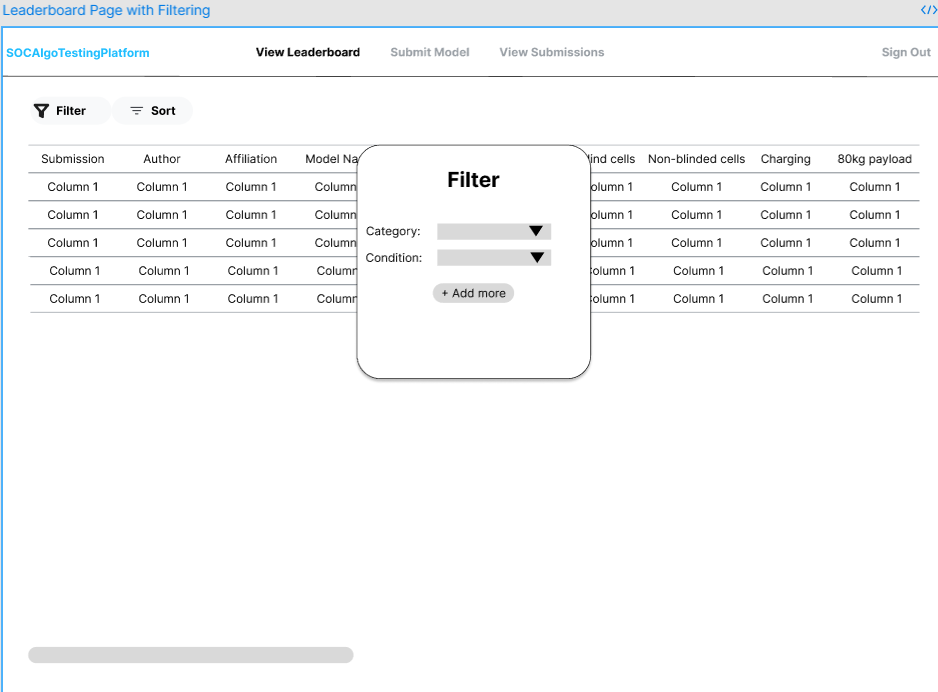
\includegraphics[width=1\linewidth]{.//Interface/Filtering.png}
\end{figure}


\bibliographystyle {plainnat}
\bibliography{../../../refs/References}

\newpage{}

\end{document}